

    \item The figures below depict two situations in which two infinitely long static line charges of constant positive line charge density $\lambda$ are kept parallel to each other. In their resulting electric field, point charges $q$ and $-q$ are kept in equilibrium between them. The point charges are confined to move in the $x$ direction only. If they are given a small displacement about their equilibrium positions, then the correct statement(s) is(are)
        \begin{center}
            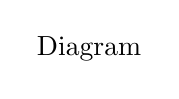
\begin{tikzpicture}
                \node {Diagram};
            \end{tikzpicture}
        \end{center}
        \begin{tasks}(1)
            \task Both charges execute simple harmonic motion.
            \task Both charges will continue moving in the direction of their displacement.
            \task Charge $+q$ executes simple harmonic motion while charge $-q$ continues moving in the direction of its displacement.
            \task Charge $-q$ executes simple harmonic motion while charge $+q$ continues moving in the direction of its displacement.
        \end{tasks}


